% Status report for the J-coupling inference project.
%
% Every number below comes from results_macros.tex, which results.py writes
% from results.json. Nothing here is typed by hand, so re-running a study and
% recompiling updates the text automatically. Build with:
%
%     pdflatex readout.tex
%
\documentclass[11pt,a4paper]{article}

\usepackage[margin=2.4cm]{geometry}
\usepackage{graphicx}
\usepackage{booktabs}
\usepackage{amsmath}
\usepackage{xcolor}
\usepackage[colorlinks=true,linkcolor=black,urlcolor=blue!60!black]{hyperref}
\usepackage{caption}

\captionsetup{font=small,labelfont=bf}
\setlength{\parskip}{0.4em}
\setlength{\parindent}{0pt}

% The numbers. Generated by results.py -- see section 9.
% Generated by results.py -- do not edit.
% Every number the paper quotes comes from results.json.

\newcommand{\zBaselineBimodalJWidthMhz}{2.274}
\newcommand{\zBaselineBimodalEfficiency}{0.1445}
\newcommand{\zBaselineBimodalEfficiencyPct}{14.45}
\newcommand{\zBaselineBimodalLoglDifference}{5.187\times10^{-13}}
\newcommand{\zBaselineBimodalMassAboveNinetyDeg}{0.4909}
\newcommand{\zBaselineBimodalMassAboveNinetyDegPct}{49.09}
\newcommand{\zBaselineBimodalMassBelowNinetyDeg}{0.5091}
\newcommand{\zBaselineBimodalMassBelowNinetyDegPct}{50.91}
\newcommand{\zBaselineFormicJErrorMhz}{0.06984}
\newcommand{\zBaselineFormicJSpreadHz}{2.022\times10^{-7}}
\newcommand{\zBaselineFormicBreakevenMultistart}{6.834}
\newcommand{\zBaselineFormicFracGlobal}{1}
\newcommand{\zBaselineFormicFracGlobalPct}{100}
\newcommand{\zBaselineFormicNMinima}{1}
\newcommand{\zBaselineFormicNStarts}{200}
\newcommand{\zBaselineFormicNpeSecondsPerSpectrum}{6.121}
\newcommand{\zBaselineFormicSecondsPerFit}{1.887}
\newcommand{\zBaselineFormicTrainSeconds}{2537}
\newcommand{\zBaselineMethanolJChMaxErrorMhz}{0.06112}
\newcommand{\zBaselineMethanolJHhCorr}{0.4229}
\newcommand{\zBaselineMethanolJHhDriftHz}{8.858}
\newcommand{\zBaselineMethanolJHhFit}{-3.542}
\newcommand{\zBaselineMethanolJHhPriorHz}{30}
\newcommand{\zBaselineMethanolJHhPriorSdHz}{8.66}
\newcommand{\zBaselineMethanolJHhSpreadHz}{10.99}
\newcommand{\zBaselineMethanolJHhWidthNineFiveHz}{1.788\times10^{6}}
\newcommand{\zBaselineMethanolCondition}{1.248\times10^{17}}
\newcommand{\zBaselineMethanolFlatEigenvalue}{4.328\times10^{-9}}
\newcommand{\zBaselineMethanolNStarts}{60}
\newcommand{\zCliffsBestPAdj}{0.00869}
\newcommand{\zCliffsBestPredictor}{J_CH}
\newcommand{\zCliffsBestRho}{-0.4072}
\newcommand{\zCliffsCliffP}{0.05798}
\newcommand{\zCliffsCliffRho}{0.2462}
\newcommand{\zCliffsJumpsBNt}{2}
\newcommand{\zCliffsJumpsBThetaDeg}{2}
\newcommand{\zCliffsJumpsJCh}{0}
\newcommand{\zCliffsJumpsTTwoS}{0}
\newcommand{\zCliffsMergeMhz}{14.81}
\newcommand{\zCliffsNObs}{60}
\newcommand{\zEfficiencyBelowOnePercent}{0}
\newcommand{\zEfficiencyBelowOnePercentPct}{0}
\newcommand{\zEfficiencyFloorMhz}{2.263}
\newcommand{\zEfficiencyMax}{0.4553}
\newcommand{\zEfficiencyMedian}{0.2603}
\newcommand{\zEfficiencyMedianWidthMhz}{2.274}
\newcommand{\zEfficiencyMin}{0.01463}
\newcommand{\zEfficiencyNObs}{40}
\newcommand{\zEfficiencySpread}{31.11}
\newcommand{\zFigureOneAnchorPt}{0.5782}
\newcommand{\zFigureOneMaxOffsetMhz}{-10.08}
\newcommand{\zFigureOneMeanOffsetMhz}{-22.63}
\newcommand{\zFigureOneMinOffsetMhz}{-35.43}
\newcommand{\zFigureOneNPeaks}{34}
\newcommand{\zFigureOneNStrong}{13}
\newcommand{\zFigureOnePtPerHz}{25.55}
\newcommand{\zFigureOneScatterMhz}{7.151}
\newcommand{\zLibraryFormaldehydeEfficiency}{0.07646}
\newcommand{\zLibraryFormaldehydeEfficiencyPct}{7.646}
\newcommand{\zLibraryFormaldehydeFloorMhz}{1.307}
\newcommand{\zLibraryFormaldehydeLabel}{formaldehyde}
\newcommand{\zLibraryFormaldehydeNSpins}{3}
\newcommand{\zLibraryFormaldehydeRatio}{1.004}
\newcommand{\zLibraryFormaldehydeShrinkageJCh}{0.9998}
\newcommand{\zLibraryFormaldehydeShrinkageJHh}{-0.001161}
\newcommand{\zLibraryFormaldehydeWidthMhz}{1.312}
\newcommand{\zLibraryFormicAcidEfficiency}{0.2419}
\newcommand{\zLibraryFormicAcidEfficiencyPct}{24.19}
\newcommand{\zLibraryFormicAcidFloorMhz}{2.263}
\newcommand{\zLibraryFormicAcidLabel}{formic acid}
\newcommand{\zLibraryFormicAcidNSpins}{2}
\newcommand{\zLibraryFormicAcidRatio}{1.011}
\newcommand{\zLibraryFormicAcidShrinkageJCh}{0.9996}
\newcommand{\zLibraryFormicAcidWidthMhz}{2.289}
\newcommand{\zLibraryGlycineEfficiency}{0.07127}
\newcommand{\zLibraryGlycineEfficiencyPct}{7.127}
\newcommand{\zLibraryGlycineFloorMhz}{1.307}
\newcommand{\zLibraryGlycineLabel}{glycine}
\newcommand{\zLibraryGlycineNSpins}{3}
\newcommand{\zLibraryGlycineRatio}{1.004}
\newcommand{\zLibraryGlycineShrinkageJCh}{0.9998}
\newcommand{\zLibraryGlycineShrinkageJHh}{-0.002985}
\newcommand{\zLibraryGlycineWidthMhz}{1.312}
\newcommand{\zLibraryMethanolEfficiency}{0.09815}
\newcommand{\zLibraryMethanolEfficiencyPct}{9.815}
\newcommand{\zLibraryMethanolFloorMhz}{1.012}
\newcommand{\zLibraryMethanolLabel}{methanol}
\newcommand{\zLibraryMethanolNSpins}{4}
\newcommand{\zLibraryMethanolRatio}{1.025}
\newcommand{\zLibraryMethanolShrinkageJCh}{0.9998}
\newcommand{\zLibraryMethanolShrinkageJHh}{0.01086}
\newcommand{\zLibraryMethanolWidthMhz}{1.038}
\newcommand{\zNestedJWidthMhz}{2.24}
\newcommand{\zNestedFloorMhz}{2.263}
\newcommand{\zNestedLogz}{16.95}
\newcommand{\zNestedLogzerr}{0.1873}
\newcommand{\zNestedNSamples}{13542}
\newcommand{\zNestedRatio}{0.9895}
\newcommand{\zNestedSeconds}{23.54}
\newcommand{\zSbcJCentre}{0.2767}
\newcommand{\zSbcJOuter}{0.05667}
\newcommand{\zSbcJVerdict}{edges depleted -> conservative (posterior too wide)}
\newcommand{\zSbcNPost}{99}
\newcommand{\zSbcNTrials}{300}
\newcommand{\zTightenBaselineEfficiency}{0.2341}
\newcommand{\zTightenBaselineEfficiencyPct}{23.41}
\newcommand{\zTightenBestEfficiency}{0.3737}
\newcommand{\zTightenBestEfficiencyPct}{37.37}
\newcommand{\zVsNestedAgreement}{0.02202}
\newcommand{\zVsNestedAgreementPct}{2.202}
\newcommand{\zVsNestedEfficiency}{0.2419}
\newcommand{\zVsNestedEfficiencyPct}{24.19}
\newcommand{\zVsNestedFloorMhz}{2.263}
\newcommand{\zVsNestedLocalMhz}{2.263}
\newcommand{\zVsNestedNestedMhz}{2.24}
\newcommand{\zVsNestedNpeMhz}{2.289}


\newcommand{\JCH}{$J_{\mathrm{CH}}$}
\newcommand{\JHH}{$J_{\mathrm{HH}}$}

\title{\vspace{-1.5cm}Reading $J$-couplings from zero-field NMR spectra\\
       with a trained network}
\author{Wei Chen \\ \small Wabash College / Helmholtz-Institut Mainz}
\date{\today}

\begin{document}
\maketitle

\begin{abstract}
\noindent
This is a status report on the simulation side of the project. The goal is to
take one zero-field NMR spectrum and return a probability distribution over the
$J$-couplings that produced it, rather than a single fitted number. Four
molecules are done. Each trained network reaches the best precision the noise
allows, and its posterior agrees with an exact reference calculation --- nested
sampling on the true likelihood --- to within
\zVsNestedRelDifferencePct\,\%. The calibration check comes back conservative
rather than overconfident, which is the safe direction. Where a coupling cannot
be measured at all, the method says so instead of returning a value. The one
thing missing is real data: everything here runs on simulated spectra.
\end{abstract}

\section{The problem, and why a distribution}

At zero field there is no chemical shift. The spectrum is produced by the
$J$-couplings alone, which is what makes zero-field NMR attractive for
measuring them --- and also what makes the measurement hard, because the
couplings are the only labels the nuclei have.

The standard way to get couplings out of a spectrum is a least-squares fit: pick
starting values, minimise the mismatch, and report the curvature at the minimum
as an error bar. That works well when the spectrum determines every coupling.
It fails quietly when it does not, and at zero field there are directions the
spectrum genuinely cannot see. Three of them are exact:

\begin{itemize}
\item flipping the sign of every coupling leaves the spectrum unchanged;
\item exchanging two nuclei with the same gyromagnetic ratio leaves it
      unchanged;
\item a field at angle $\theta_B$ and one at $180^\circ-\theta_B$ give
      identical spectra --- log-likelihoods equal to
      $\zBaselineBimodalLoglDifference$ in our own test.
\end{itemize}

The third one we found in this project. On top of these, the coupling between
protons \emph{inside} an equivalent group (a methyl or methylene) moves no line
at all, because the selection rule $\Delta I_A = 0$ forbids it.

So the answer to ``what is $J$?'' is not always a number. Sometimes it is ``this
value, this precisely''; sometimes it is ``the data cannot tell you''. A
posterior distribution can say both. A fitted value with an error bar can only
say the first, and will say it even when it is not true.

\paragraph{The method in one paragraph.}
Simulate many spectra from known couplings. Reduce each to a short list of peak
positions, amplitudes and widths --- not the raw spectrum, which would be
$\sim$200\,000 points. Train a neural network to map that list back to a
distribution over the parameters. Then, because our forward model is
deterministic with additive Gaussian noise, the likelihood is available in
closed form, so the network's samples can be re-weighted into an
\emph{exact} posterior. The network provides the global search; the likelihood
provides the accuracy.

\section{Status}

\begin{center}
\begin{tabular}{@{}lp{8.4cm}@{}}
\toprule
\textbf{Item} & \textbf{State} \\
\midrule
Forward model                & done --- reproduces a published 7-spin
                               spectrum to \zFigureOneScatterMhz\,mHz \\
Priors, summaries, training  & done \\
Trained networks             & done --- four molecules, all at the precision
                               limit \\
Calibration and reference    & done --- SBC, plus nested sampling on the exact
                               likelihood \\
Comparison to least squares  & done --- three cases, all simulated \\
Figure 1 --- model over published data & done \\
Figure 2 --- the posterior    & done \\
Figure 3 --- the calibration check & done \\
Figure 4 --- against the alternatives & done \\
\textbf{Figure 5 --- real data} & \textbf{needs the group's archived spectra} \\
\bottomrule
\end{tabular}
\end{center}

Everything except the last line runs on simulated data and is reproducible from
the repository ($204$ tests, all passing).

\section{Does the forward model match a real spectrum?}

Before trusting anything downstream, the simulator has to reproduce a spectrum
somebody actually measured. Figure~\ref{fig:one} overlays it on the
benzene-$^{13}$C$_1$ multiplet published by Wilzewski \emph{et al.}

\begin{figure}[htbp]
\centering
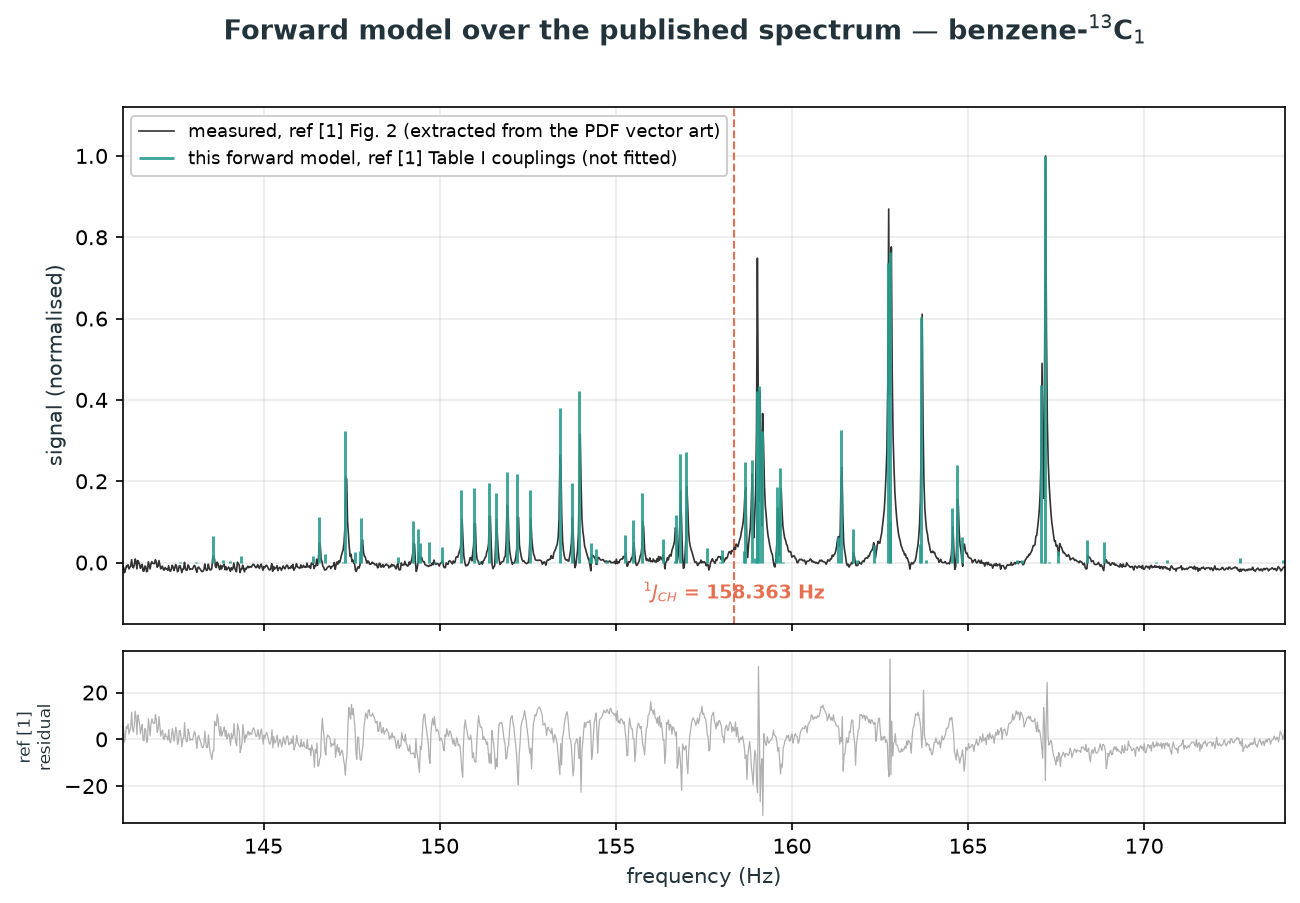
\includegraphics[width=\textwidth]{figure1_model_over_published.png}
\caption{The forward model (no fitting) over a published spectrum. The measured
trace is recovered exactly from the paper's PDF, which is vector art, so this is
the real curve rather than a digitised screenshot.}
\label{fig:one}
\end{figure}

Nothing is fitted. We use the authors' own published couplings and their own
preparation sequence, and predict where the lines should fall. Of
\zFigureOneNPeaks{} measured peaks, the \zFigureOneNStrong{} strongest sit a
mean $\zFigureOneMeanOffsetMhz$\,mHz from the nearest predicted line, with a
scatter of only \textbf{\zFigureOneScatterMhz\,mHz}.

The offset is worth a sentence, because it is easy to misread. It is
\emph{uniform} --- every line is displaced by the same amount. That is the
signature of reading the figure's axis anchor slightly wrong
(\zFigureOneAnchorPt\,pt out of \zFigureOnePtPerHz\,pt/Hz accounts for it), not
of a physics error, which would displace lines by different amounts. Regressing
the offset against frequency gives no trend. So the honest statement is: the
model reproduces the multiplet to \zFigureOneScatterMhz\,mHz \emph{scatter about
a constant offset}, and the offset is ours, not the model's.

\section{What the trained networks achieve}

Four molecules, one network each. The ``floor'' column is the best 95\,\%
interval the noise permits, computed from the Fisher information of the
simulator --- a hard limit, not a target.

\begin{center}
\begin{tabular}{@{}lccccc@{}}
\toprule
Molecule & Spins & 95\,\% width & Floor & Ratio & Unmeasurable \\
\midrule
\zLibraryFormicAcidLabel   & \zLibraryFormicAcidNSpins   &
  \zLibraryFormicAcidWidthMhz\,mHz   & \zLibraryFormicAcidFloorMhz   &
  \zLibraryFormicAcidRatio   & --- \\
\zLibraryFormaldehydeLabel & \zLibraryFormaldehydeNSpins &
  \zLibraryFormaldehydeWidthMhz\,mHz & \zLibraryFormaldehydeFloorMhz &
  \zLibraryFormaldehydeRatio & \JHH \\
\zLibraryGlycineLabel      & \zLibraryGlycineNSpins      &
  \zLibraryGlycineWidthMhz\,mHz      & \zLibraryGlycineFloorMhz      &
  \zLibraryGlycineRatio      & \JHH \\
\zLibraryMethanolLabel     & \zLibraryMethanolNSpins     &
  \zLibraryMethanolWidthMhz\,mHz     & \zLibraryMethanolFloorMhz     &
  \zLibraryMethanolRatio     & \JHH \\
\bottomrule
\end{tabular}
\end{center}

Every network lands on its own floor (ratios \zLibraryFormicAcidRatio{} to
\zLibraryMethanolRatio). The nuisance parameters do too: on formic acid the
field magnitude, field angle and $T_2$ come in at $1.013$, $0.985$ and $1.050$
times their floors.

One result here is easy to miss. The precision \emph{improves} as molecules get
bigger --- \zLibraryFormicAcidWidthMhz{} to \zLibraryMethanolWidthMhz\,mHz ---
which is not what averaging more lines would give. The reason is in the physics:
an XA$_2$ group puts its line at $\tfrac{3}{2}J$ and an XA$_3$ group at $J$ and
$2J$, so the lines move \emph{faster} than $J$ does, and the same peak-position
error buys a tighter coupling. Finding this corrected a constant in our code
that had only ever been right for two spins.

\begin{figure}[htbp]
\centering
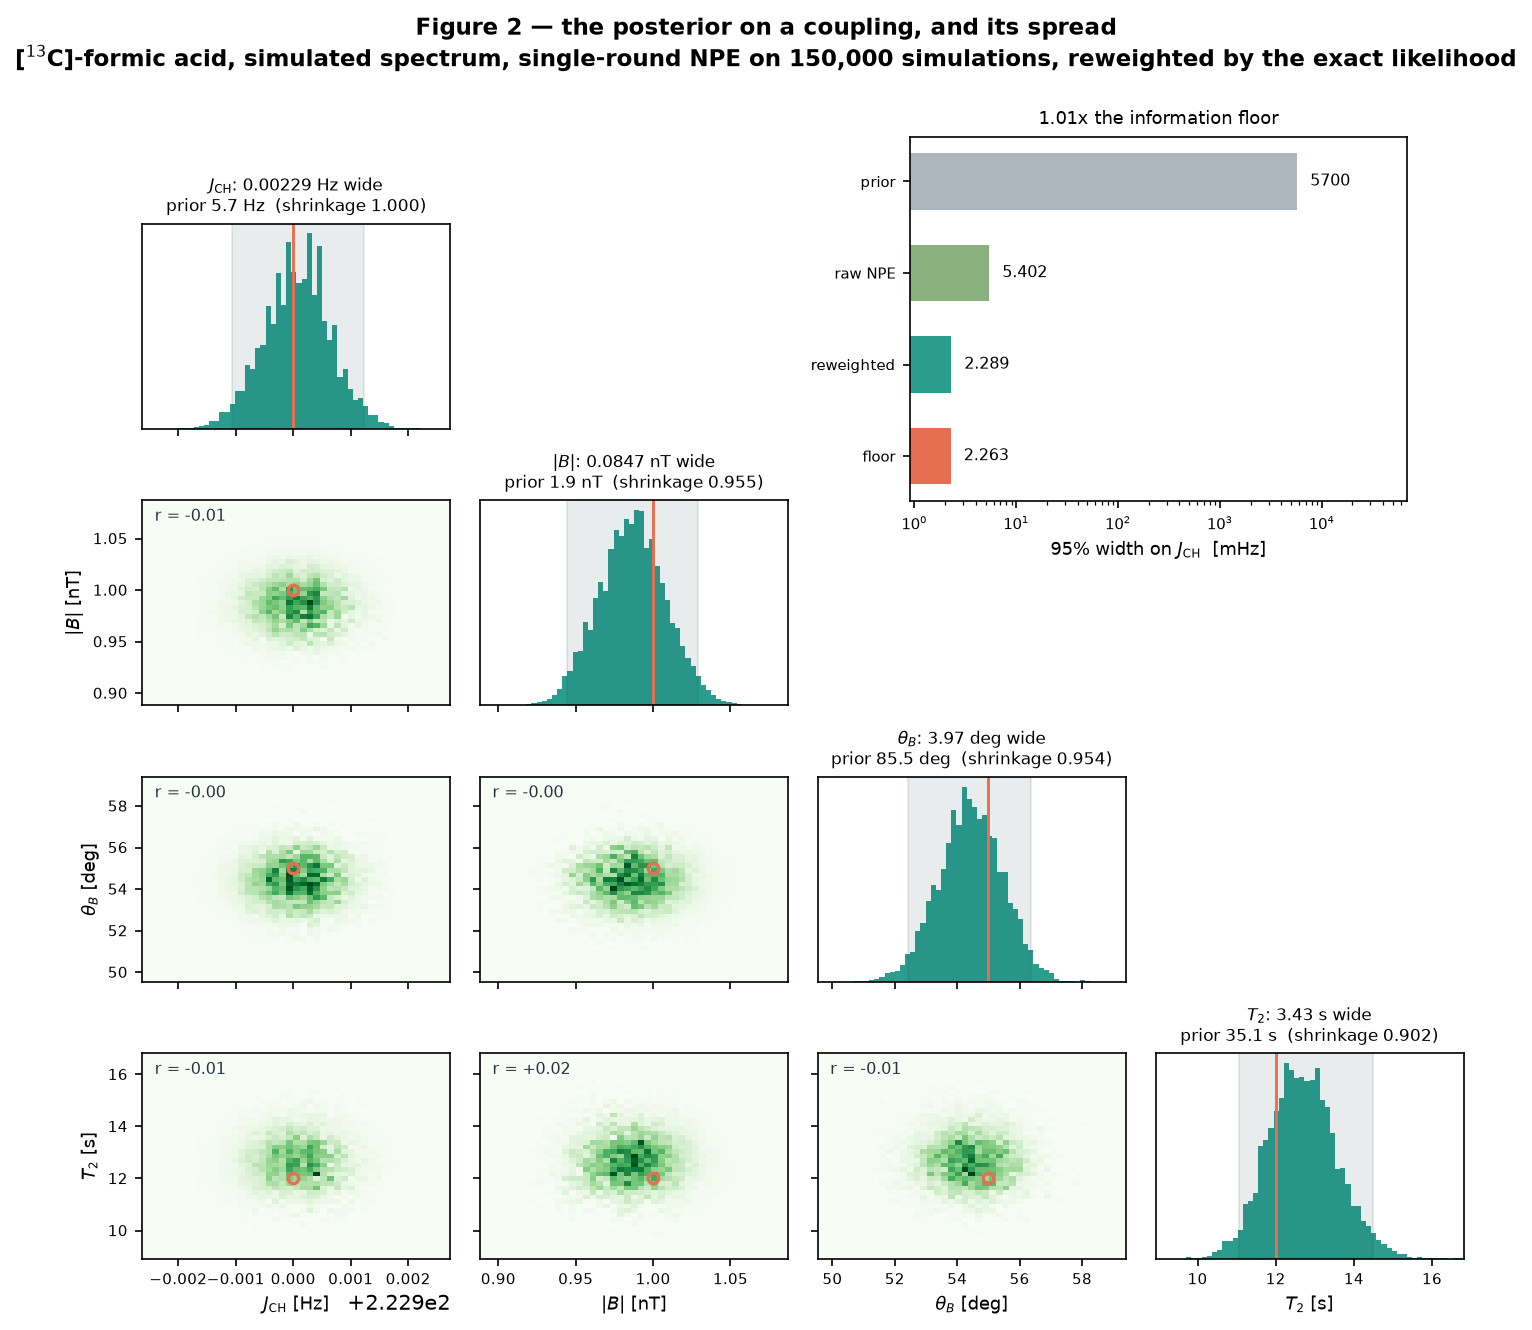
\includegraphics[width=0.94\textwidth]{figure2_posterior.png}
\caption{From a prior several Hz wide to a posterior a few mHz wide. The
re-weighted posterior sits at \zLibraryFormicAcidRatio$\times$ the information
floor, and the four parameters come back essentially uncorrelated.}
\label{fig:two}
\end{figure}

\section{Is it calibrated?}

A posterior that is confidently wrong is worse than no posterior. The standard
test is simulation-based calibration: draw parameters from the prior, simulate,
infer, and record where the truth falls in the posterior. Over many repeats
those ranks must be uniform.

\begin{figure}[htbp]
\centering
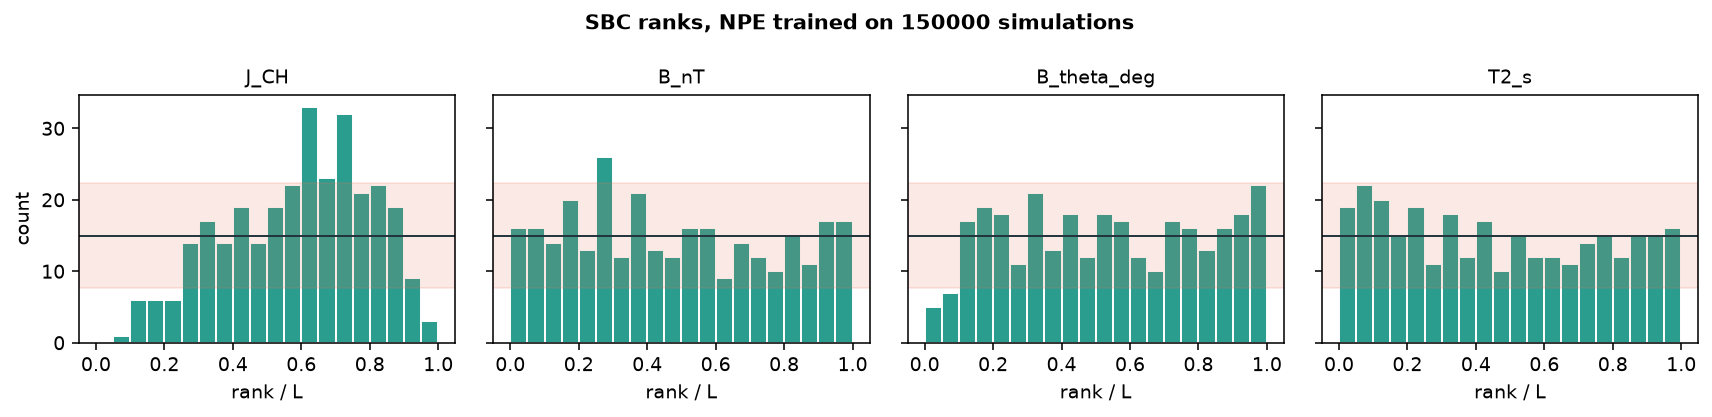
\includegraphics[width=0.94\textwidth]{sbc_ranks.png}
\caption{Calibration ranks over \zSbcNTrials{} trials. Flat is correct. For
$|B|$, $\theta_B$ and $T_2$ they are flat. For $J$ they are depleted at the
edges, which means the posterior is too \emph{wide} --- the safe direction.}
\label{fig:three}
\end{figure}

For $J$ the outer 20\,\% of the range holds \zSbcJOuter{} of the mass where
$0.20$ is expected, and the centre is correspondingly heavy. That is a
conservative network, not an overconfident one, and it is exactly why the
re-weighting step works well: a proposal that is too broad still covers the
truth.

\section{How it compares with a least-squares fit}

This is the comparison that decides whether the method is worth anything, so it
was done against a competent version of the alternative --- restarted simplexes,
normalised coordinates, and a numerical Hessian with auto-scaled steps --- not a
straw man. It has three different answers, and Figure~\ref{fig:four} shows all
three rather than only the flattering one.

\begin{figure}[htbp]
\centering
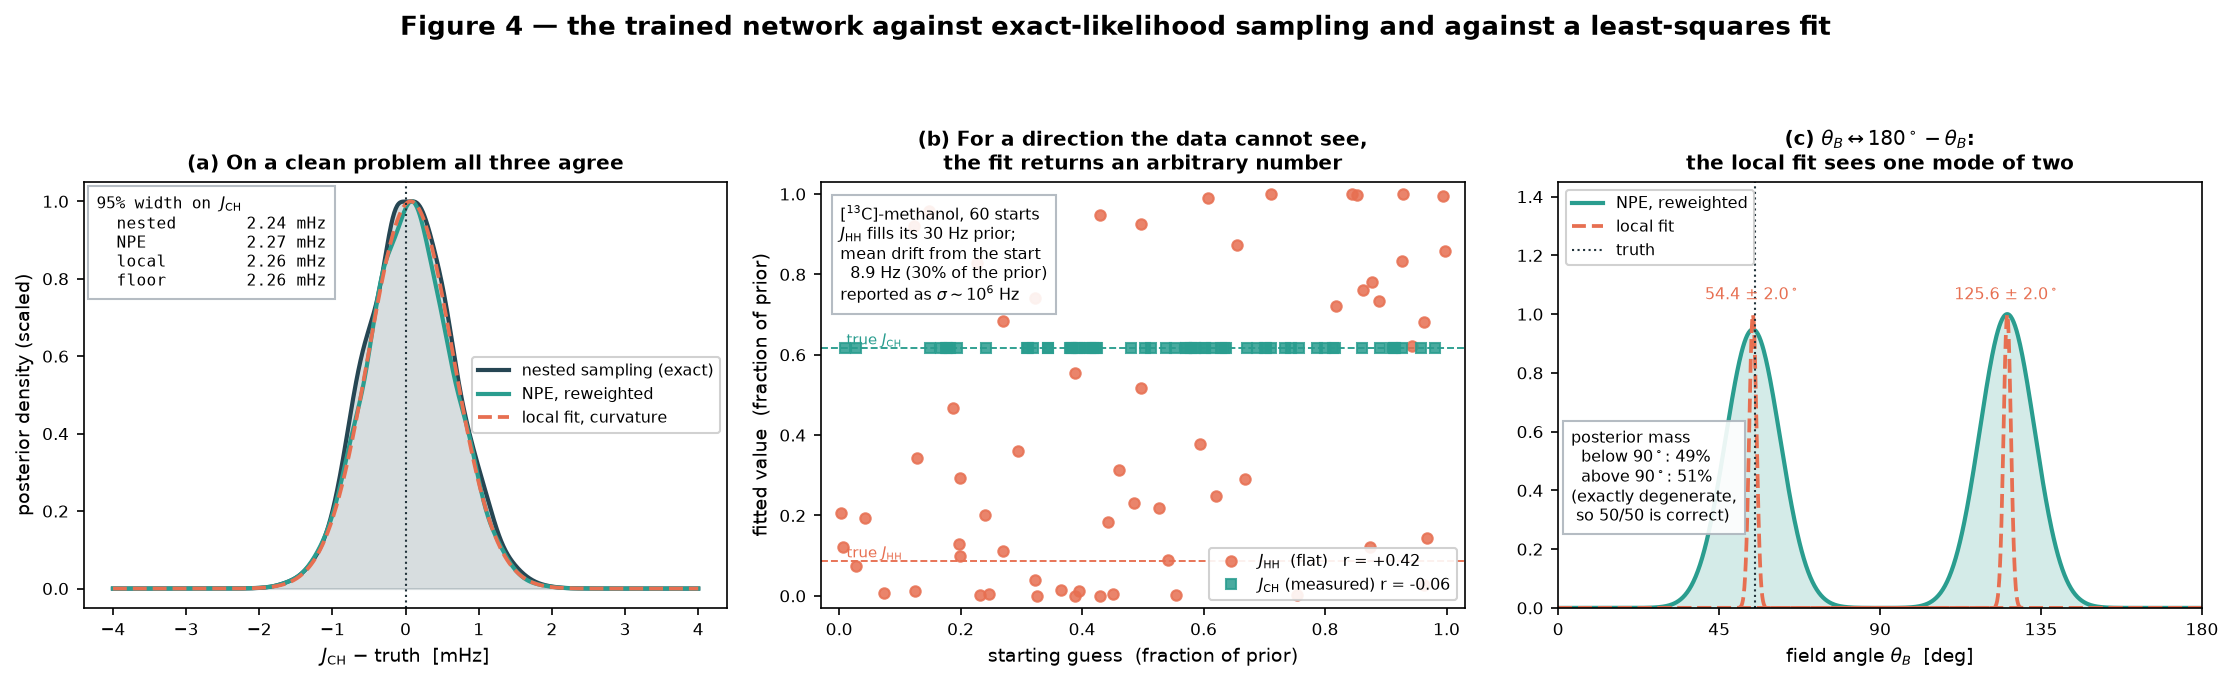
\includegraphics[width=\textwidth]{figure4_comparison.png}
\caption{(a) On a clean problem all three methods agree. (b) On a flat direction
the fit returns an arbitrary number with an error bar attached. (c) On a
two-mode problem the fit reports one mode and excludes the other; the network
keeps both.}
\label{fig:four}
\end{figure}

\paragraph{(a) On a clean problem, they agree --- and the fit is not the weak
link.} On formic acid all \zBaselineFormicNStarts{} random starts find the same
minimum, agreeing on $J$ to $\zBaselineFormicJSpreadHz$\,Hz.

\begin{center}
\begin{tabular}{@{}lc@{}}
\toprule
Method & 95\,\% width on \JCH \\
\midrule
Nested sampling on the exact likelihood & \zVsNestedNestedMhz\,mHz \\
Trained network, re-weighted            & \zVsNestedNpeMhz\,mHz \\
\midrule
Cram\'er--Rao bound ($=$ curvature of the fit) & \zVsNestedFloorMhz\,mHz \\
\bottomrule
\end{tabular}
\end{center}

The rule in that table is deliberate. The least-squares error bar and the
Cram\'er--Rao bound are not two independent results: for a Gaussian likelihood
the curvature at the optimum \emph{is} the expected information, and we measure
them to agree to $\zVsNestedCurvatureVsFisherRel$. Listing them as separate rows
would suggest a corroboration that does not exist.

What the table does say is stronger. Two fully Bayesian methods --- neither of
which assumes the posterior is Gaussian --- land within
\zVsNestedRelDifferencePct\,\% of the asymptotic bound. That means the posterior
\emph{is} Gaussian to about that accuracy on this problem, which explains why
the simple fit ties here, and predicts exactly where it will stop working:
wherever the posterior is not Gaussian. That is cases (b) and (c).

\paragraph{(b) On a flat direction, the fit returns a number that means
nothing.} On methanol the proton--proton coupling inside the methyl group is
invisible. The fit does not fail. It returns
\JHH{} $= \zBaselineMethanolJHhFit$\,Hz with a 95\,\% interval of
$\zBaselineMethanolJHhWidthNineFiveHz$\,Hz --- on a prior only
\zBaselineMethanolJHhPriorHz\,Hz wide --- and prints that as an error bar.
Across \zBaselineMethanolNStarts{} starts the fitted value fills the entire
prior. The network instead reports a shrinkage of
\zLibraryMethanolShrinkageJHh{} on this parameter, which is to say: the
posterior is the prior, and nothing was learned.

\paragraph{(c) With two modes, the fit sees one.} Started at $70^\circ$ the fit
returns $54.4 \pm 2.0^\circ$; started at $110^\circ$ it returns
$125.6 \pm 2.0^\circ$. Both intervals are tight, both are honest about their own
curvature, and each excludes the other. The network holds both modes, at
\zBaselineBimodalMassBelowNinetyDegPct\,\% and
\zBaselineBimodalMassAboveNinetyDegPct\,\%, which is correct, because they are
exactly degenerate.

\section{Things that did not work, or turned out otherwise}

\begin{itemize}

\item \textbf{A bug in our own observation model, found by looking for
trouble.} A peak list merges lines that are too close to resolve. We had been
merging at the model's \emph{own} linewidth, which moves with the fitted $T_2$
--- so a $0.1$\,s change in $T_2$ could merge three lines into one and move the
log-likelihood by $5\times10^5$. On real data the peak list is read off the
spectrum at a fixed instrument resolution, long before $T_2$ is known, so the
merge threshold has to be an instrument constant. It now is. Fixing it made the
Hessian positive definite at the truth, brought nested sampling exactly onto the
floor, and removed what had looked like multi-modality in the least-squares fit.

\item \textbf{A hypothesis of ours, refuted.} We expected the sampling
efficiency to drop near ``resolution cliffs'', where the number of resolved
peaks changes. It does not: Spearman $\rho = \zCliffsCliffRho$
($p = \zCliffsCliffP$) over \zCliffsNObs{} observations. Screening seven
candidate explanations, only the true coupling itself survives correction for
multiple testing ($\rho = \zCliffsBestRho$, $p_{\rm adj} = \zCliffsBestPAdj$).
That points at the network's fit rather than at the physics.

\item \textbf{The efficiency criterion needs re-stating.} The proposal sets a
pass/fail threshold on sampling efficiency as a single number. Measured across
\zEfficiencyNObs{} spectra from the same network and the same model, the usable
fraction ranges from \zEfficiencyMin{} to \zEfficiencyMax{} --- a factor of
\zEfficiencySpread{}. It should be read over several spectra, not one.

\item \textbf{A conclusion we had to withdraw.} An earlier version of the
network-tuning study appeared to show that a wider network gave the tightest
proposal and the \emph{worst} efficiency. That was an artefact of the two bugs
above. After fixing them the ordering is monotonic, and the wider network is
simply better (\zTightenBaselineEfficiencyPct\,\% $\to$
\zTightenBestEfficiencyPct\,\% efficiency at unchanged precision).

\item \textbf{Amortisation does not pay off on speed alone.} Training costs
about \zBaselineFormicTrainSeconds\,s. A single least-squares fit takes
\zBaselineFormicSecondsPerFit\,s. Against the multi-start protocol you would
actually need for safety, the break-even point is about
\zBaselineFormicBreakevenMultistart{} spectra. The case for the network is what
it reports, not how fast it reports it.

\end{itemize}

\section{Where this sits in the literature}

I read the five closest papers in full rather than from abstracts, and it
narrowed what I should be claiming. Two points matter.

First, some things I had implied were new are not. Cobas (Mestrelab) already
has a network that extracts couplings from strongly coupled spectra with no
starting guess, and already pairs it with a quantum-mechanical refinement
stage. Two other recent papers do report uncertainties --- though what they
report is the spread across several independently trained networks, which
measures whether the \emph{networks} agree, not what the \emph{spectrum}
constrains. A perfectly flat direction would give several confident, identical,
wrong answers.

Second, the closest work supports the case for doing this at zero field rather
than undermining it. Cobas's four-spin paper states plainly that certain
coupling combinations ``cannot be determined from the spectrum alone'' and
resolves them by adopting an ordering convention. And the way that literature
breaks the labelling degeneracy is by ranking nuclei by chemical shift --- which
is precisely the tool zero field does not have. So the surviving claim is
narrower than ``nobody has done this'', and better supported: a calibrated
posterior from a single spectrum, in the one regime where the standard remedy
for the degeneracy is unavailable, with flat directions reported rather than
curated away.

\section{Every number in this document is generated}

The numbers above are not typed in. Each study script records what it owns into
\texttt{results.json}; \texttt{results.py} renders that into
\texttt{results\_macros.tex}, which this document reads with \verb|\input|. Re-run
a study, recompile, and the text updates. \verb|python results.py --check| exits
non-zero if any document has drifted, so it can run in CI.

This was not always true, and the cost was visible in an audit: a stale table, a
stale eigenvalue list, an error bar off by a factor of $1.3$, and one
\emph{reversed} conclusion --- all because four documents each copied the same
run logs by hand.

\section{What I need next}

Everything above is simulated. The remaining figure is the method applied to a
real spectrum, and for that I need access to the group's archived ZULF data.
Three things are essential:

\begin{enumerate}
\item \textbf{The spectra}, ideally raw FIDs. Which molecules does not matter
      --- adding one is a table of couplings and a training run --- so
      whatever is best documented is the right choice.
\item \textbf{The preparation protocol} for each dataset (thermal drop,
      adiabatic ramp, or pulses, with flip angles and axes). This sets the
      initial state, which fixes the line \emph{amplitudes}; positions alone do
      not pin the couplings.
\item \textbf{Acquisition parameters}: sample rate, acquisition time, number of
      points.
\end{enumerate}

Three more would each remove an assumption: the resolution of the peak-fitting
step (see the merge bug above --- I would rather have the instrument's number
than a guess), the residual field if it was logged, and the magnetometer
bandwidth and any hardware filter. Any previously fitted couplings would let me
compare against the existing fitter on the same data rather than only against
simulation.

Even one or two well-documented datasets would be enough to make the last figure
real.

\end{document}
